\section{与经典积分的关系}
\label{sec:integral-classical}

一般积分已经有了定义和运算规则，现在把它与此前熟悉的累计方式逐一对应。离散求和对每个点按权重累加；闭区间上的黎曼积分用分割与上下和夹逼；反常积分在黎曼积分之外再取一次截断极限。这三者在\BookChapterRef{chap:univariate-integration}{卷1《数学准备：基础数学》的“一元函数的积分”章}与该卷的级数讨论中已经建立，本节使用其中的Darboux判据（有界函数黎曼可积当且仅当上下和之差可以任意小）、反常积分的截断定义与$\int_1^{+\infty}\sin x/x\,\mathrm dx$的收敛性，逐项说明它们在什么条件下与测度积分一致，又在哪里分道扬镳。

\subsection{与离散求和的关系}
\label{sec:integral-discrete-sums}

\paragraph{非负加权和}
设$X$是有限集或可数集，$\mathcal A$为$X$的全部子集，给每个点一个权重$w(x)\in[0,+\infty]$，令$\mu(A)=\sum_{x\in A}w(x)$。由引理~\ref{lem:measure-weighted-sum}，$\mu=\sum_xw(x)\delta_x$是测度；$w\equiv1$时就是计数测度。非负项的和不依赖求和次序，其值是全部有限部分和的上确界，可以为$+\infty$。

\begin{theorem}[离散测度上的积分即加权和]
\label{thm:integral-discrete-sum}
在上述设定下，对任意$f:X\to[0,+\infty]$，
\[
 \int_Xf\,\mathrm d\mu=\sum_{x\in X}f(x)\,w(x).
\]
对实值或复值$f$，$f$为$\mu$-可积当且仅当$\sum_x|f(x)|w(x)<+\infty$，此时$\int_Xf\,\mathrm d\mu=\sum_xf(x)w(x)$，右端级数绝对收敛，其和与求和次序无关。
\end{theorem}

\begin{proof}
所有子集都可测，所以每个函数都可测。先看单点：对$c\in[0,+\infty]$，$\int c\mathbf 1_{\{x\}}\,\mathrm d\mu=c\,w(x)$。$c$有限时这是简单函数的积分；$c=+\infty$时，若$w(x)=0$，由引理~\ref{lem:integral-nonnegative-basic}第3条积分为零，若$w(x)>0$，对每个$M$积分都不小于$Mw(x)$，故为$+\infty$，与约定$(+\infty)\cdot w(x)$一致。

把$X$排成$x_1,x_2,\dots$（有限时只有有限项），令$f_N=\sum_{k\le N}f(x_k)\mathbf 1_{\{x_k\}}$。由非负积分的加法，$\int f_N=\sum_{k\le N}f(x_k)w(x_k)$。$f_N$在每一点从某项起等于$f$，且逐点递增，单调收敛定理给出$\int f=\lim_N\sum_{k\le N}f(x_k)w(x_k)$，这就是非负级数的和。

对实值$f$，把结论用于$|f|$得到可积性的刻画；可积时对$f^+$、$f^-$分别使用，两个非负级数都有限，相减得到$\sum_xf(x)w(x)$。绝对收敛级数可以拆成正项与负项之差，并可任意重排而和不变，所以右端与次序无关。复值情形对实部和虚部分别处理。
\end{proof}

于是离散累计中的“权重”正是所选测度在各点上的质量。在$\mathbb N=\{1,2,\dots\}$上取计数测度，$f(k)=2^{-k}$的积分为$\sum_k2^{-k}=1$。图~\ref{fig:integral-counting-measure-series}左侧把每一点画成质量为$1$、高为$f(k)$的柱，右侧画出截断函数$f_N$的积分$1-2^{-N}$，它们正是证明中单调收敛定理所用的递增列。换成权重$w(k)=2^{-k}$，函数$f(k)=k$的积分为$\sum_kk2^{-k}=2$，这是由$\sum_kkx^k=x/(1-x)^2$在$x=\tfrac12$处取值得到的。

\begin{figure}[!htbp]
 \centering
 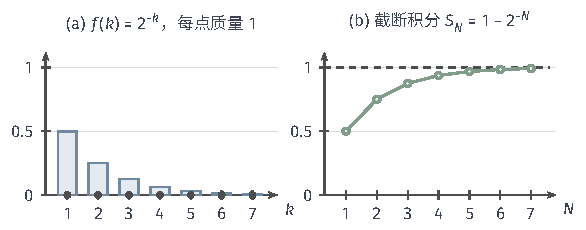
\includegraphics[width=99.24mm]{figures/02-abstract-mathematics/01-metric-and-measure/tikz/c3-counting-measure-series/figure.pdf}
 \caption{计数测度下的积分即级数。(a)$\mathbb N$上每一点（黑点）的质量为$1$，柱高为$f(k)=2^{-k}$，图中画出$k=1,\dots,7$。(b)截断$f_N=f\mathbf 1_{\{1,\dots,N\}}$的积分$S_N=1-2^{-N}$随$N$递增并趋于$1$，与单调收敛定理给出的$\int f=1$一致。}
 \label{fig:integral-counting-measure-series}
\end{figure}

\paragraph{条件收敛级数不对应积分}
定理把有限积分对应到\emph{绝对}可和，而不是对应到某种次序下收敛的级数。以$f(k)=(-1)^{k+1}/k$为例，级数$\sum_k(-1)^{k+1}/k$按原次序收敛（第~\ref{sec:integral-limits-dominated}小节将用控制收敛定理求出它的和为$\log2$），但$\sum_k|f(k)|$是发散的调和级数，所以$f$对计数测度不可积。进一步，$\int f^+=\sum_j\frac1{2j-1}$与$\int f^-=\sum_j\frac1{2j}$都是$+\infty$，$f$的积分甚至不存在。

这不是定义上的缺陷，而是测度积分不依赖次序这一要求的必然结果。计数测度上的积分是对集合$\mathbb N$赋值，集合没有“先后”；而由卷1中级数重排的讨论，条件收敛级数经过重排可以收敛到任意预先指定的实数。若把某一种次序下的和当作积分，就要在同一个测度下为同一个函数选定一种排列，这与测度的可数可加性对次序无关相矛盾。

\subsection{与黎曼积分的关系}
\label{sec:integral-riemann}

\paragraph{区间与阶梯函数}
对区间$I\subseteq[a,b]$（开、闭或半开），$\int\mathbf 1_I\,\mathrm d\lambda=\lambda(I)$等于区间长度，这与黎曼积分的值相同。端点只是零测集，开闭不影响Lebesgue积分；黎曼积分同样不受有限个点上取值的影响。由两种积分的线性，阶梯函数$\varphi=\sum_ic_i\mathbf 1_{I_i}$（$I_i$为区间）的两种积分都等于$\sum_ic_i\lambda(I_i)$。黎曼积分的上下和正是阶梯函数的积分，下面的定理就从这里把两种理论连起来。

\paragraph{Lebesgue判据}
判别有界函数是否黎曼可积，需要量化函数在一点附近的跳动幅度。设$f:[a,b]\to\mathbb R$有界，记$I_\delta(x)=(x-\delta,x+\delta)\cap[a,b]$，定义$f$在$x$处的\term{振幅}（oscillation）
\[
 \omega_f(x)=\inf_{\delta>0}\Bigl(\sup_{I_\delta(x)}f-\inf_{I_\delta(x)}f\Bigr).
\]
括号内的量随$\delta$减小而不增。$f$在$x$连续当且仅当$\omega_f(x)=0$：若连续，给定$\varepsilon$，取$\delta$使$I_\delta(x)$上$|f(y)-f(x)|<\varepsilon/2$，则括号内的量不超过$\varepsilon$；反之若$\omega_f(x)=0$，对给定$\varepsilon$取$\delta$使括号内的量小于$\varepsilon$，则$I_\delta(x)$上$|f(y)-f(x)|<\varepsilon$。于是不连续点集为$D_f=\bigcup_{m\ge1}\{\omega_f\ge1/m\}$。

\begin{theorem}[黎曼可积的Lebesgue判据]
\label{thm:integral-riemann-lebesgue}
设$f:[a,b]\to\mathbb R$有界。$f$黎曼可积，当且仅当其不连续点集$D_f$是Lebesgue零测集。此时$f$对Lebesgue可测集构成的$\sigma$代数可测，Lebesgue可积，且$\int_{[a,b]}f\,\mathrm d\lambda=\int_a^bf(x)\,\mathrm dx$。
\end{theorem}

这一判据称为\term{Lebesgue判据}（Lebesgue criterion）。证明分三步：先说明黎曼可积函数的两种积分相等，并在同一过程中得到$D_f$零测；再由$D_f$零测构造上下和之差很小的分割。设$|f|\le M$。

\begin{proof}
\emph{第一步：黎曼可积函数的Lebesgue积分。}设$f$黎曼可积。由Darboux判据，对每个$k$有分割$Q_k$使上下和之差小于$1/k$；令$P_k$为$Q_1,\dots,Q_k$的公共加细，加细不增大上下和之差，于是$P_1\subseteq P_2\subseteq\cdots$且$U(f,P_k)-L(f,P_k)\to0$。对分割$P_k$的每个小段$[x_{i-1},x_i]$，记$m_i,M_i$为$f$在其上的下、上确界，令
\[
 \varphi_k=\sum_im_i\mathbf 1_{J_i},\qquad\psi_k=\sum_iM_i\mathbf 1_{J_i},
\]
其中$J_i=[x_{i-1},x_i)$，最后一段取闭区间。于是$\varphi_k\le f\le\psi_k$处处成立，$\int\varphi_k\,\mathrm d\lambda=L(f,P_k)$，$\int\psi_k\,\mathrm d\lambda=U(f,P_k)$。分割加细时子段上的下确界不减、上确界不增，所以$\varphi_k$递增、$\psi_k$递减，分别有逐点极限$\varphi\le f\le\psi$，它们是Borel可测函数。

由$0\le\psi-\varphi\le\psi_k-\varphi_k$，$\int(\psi-\varphi)\le U(f,P_k)-L(f,P_k)\to0$，故$\int(\psi-\varphi)=0$，由引理~\ref{lem:integral-nonnegative-basic}第4条，$\psi=\varphi$在零测集$N$外成立，从而$f=\varphi$在$N$外成立。对任意$t$，$\{f>t\}$与Borel集$\{\varphi>t\}$只在$N$内可能不同；$(\mathbb R,\mathcal L,\lambda)$完备，所以$f$对$\mathcal L$可测。又$|f|\le M$且区间测度有限，$f$可积。$\varphi_k+M\ge0$递增到$\varphi+M$，单调收敛定理给出$\int(\varphi_k+M)\to\int(\varphi+M)$，两边减去有限数$M(b-a)$得
\[
 \int_{[a,b]}f\,\mathrm d\lambda=\int_{[a,b]}\varphi\,\mathrm d\lambda=\lim_kL(f,P_k)=\int_a^bf(x)\,\mathrm dx.
\]

\emph{第二步：黎曼可积蕴含$D_f$零测。}全部分割$P_k$的分点只有可数个，组成零测集$Z$。若$x\notin Z$，对每个$k$，$x$位于$P_k$某个小段的内部，存在$\delta$使$I_\delta(x)$包含于该小段，于是$\omega_f(x)\le M_i-m_i=\psi_k(x)-\varphi_k(x)$。令$k\to\infty$得$\omega_f(x)\le\psi(x)-\varphi(x)$。在零测集$Z\cup N$之外右端为零，所以$D_f=\{\omega_f>0\}\subseteq Z\cup N$，是零测集。

\emph{第三步：$D_f$零测蕴含黎曼可积。}给定$\varepsilon>0$，令$K=\{\omega_f\ge\varepsilon\}$。$K$是闭集：若$\omega_f(x)<\varepsilon$，取$\delta$使$I_\delta(x)$上上下确界之差小于$\varepsilon$，则对$|y-x|<\delta/2$，$I_{\delta/2}(y)\subseteq I_\delta(x)$，故$\omega_f(y)<\varepsilon$，即$\{\omega_f<\varepsilon\}$在$[a,b]$中相对开。$K\subseteq D_f$是零测的有界闭集，由外测度的定义可用可数个开区间覆盖$K$且总长小于$\varepsilon$；$K$紧致，取其中有限个，记其并为$G$，它由有限个两两不交的开区间组成，总长小于$\varepsilon$。

$[a,b]\setminus G$是有限个闭区间$H_1,\dots,H_r$之并，其上处处$\omega_f<\varepsilon$。对每点$x\in H_l$取$\delta_x$使$I_{\delta_x}(x)$上的上下确界之差小于$\varepsilon$；区间$(x-\delta_x/2,x+\delta_x/2)$覆盖紧集$H_l$，取有限子覆盖，令$\delta$为相应$\delta_x/2$的最小值。若$H_l$中的小段$J$长度小于$\delta$，取$y\in J$，$y$落在某个$(x-\delta_x/2,x+\delta_x/2)$中，则$J\subseteq I_{\delta_x}(x)$，$f$在$J$上的上下确界之差小于$\varepsilon$。把每个$H_l$分成长度小于$\delta$的小段，再加上$G$各分支与$[a,b]$之交的端点，得到分割$P$。$P$的小段分两类：落在某个$H_l$中的，上下确界之差小于$\varepsilon$，总长不超过$b-a$；落在$G$某个分支闭包中的，上下确界之差不超过$2M$，总长小于$\varepsilon$。所以
\[
 U(f,P)-L(f,P)<\varepsilon(b-a)+2M\varepsilon,
\]
由$\varepsilon$的任意性与Darboux判据，$f$黎曼可积。
\end{proof}

第一步说明两种理论在共同范围内一致：黎曼可积函数的上下阶梯函数从两侧夹住它，Lebesgue积分只是记录了夹逼的公共极限。第二、三步说明黎曼可积的障碍恰好是不连续点占据正的长度。这里用到完备性：$f$未必Borel可测，但与Borel函数仅在零测集上不同。

\paragraph{Dirichlet函数}
在$[0,1]$上，有理点示性函数$\mathbf 1_{\mathbb Q}$称为\term{Dirichlet函数}（Dirichlet function）。$\mathbb Q\cap[0,1]$可数，Lebesgue测度为零，所以$\int_{[0,1]}\mathbf 1_{\mathbb Q}\,\mathrm d\lambda=0$。另一方面，有理点与无理点都在$[0,1]$中稠密，每个小区间上$\mathbf 1_{\mathbb Q}$的上确界为$1$、下确界为$0$，振幅处处为$1$，$D_f=[0,1]$的测度为$1$，由Lebesgue判据它不黎曼可积；这与卷1中“任意分割的下和为$0$、上和为$1$”的计算一致。图~\ref{fig:integral-dirichlet-function}(a)用两条点线示意这种处处跳动。

\begin{figure}[!htbp]
 \centering
 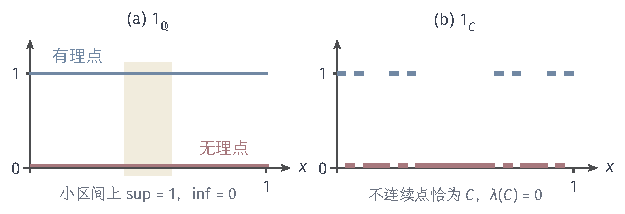
\includegraphics[width=105.876mm]{figures/02-abstract-mathematics/01-metric-and-measure/tikz/c3-dirichlet-function/figure.pdf}
 \caption{两种不连续点集。(a)Dirichlet函数$\mathbf 1_{\mathbb Q}$在有理点取$1$（蓝）、无理点取$0$（红），两类点都稠密，任一小区间（黄色带）上上确界为$1$、下确界为$0$，不连续点集为整个$[0,1]$。(b)Cantor集示性函数$\mathbf 1_C$，用第三步的$8$个保留区间示意$C$；它在$C$外的开区间上恒为零而连续，不连续点恰为$C$，$\lambda(C)=0$，所以黎曼可积且积分为$0$。}
 \label{fig:integral-dirichlet-function}
\end{figure}

这个例子同时区分了稠密与零测：$\mathbb Q\cap[0,1]$稠密却零测，函数在它上面的取值对Lebesgue积分毫无影响，对黎曼积分却是致命的，因为黎曼上下和在每个小区间上都会“看到”有理点。图(b)给出另一侧的对照。Cantor集$C$（例~\ref{ex:measure-cantor-set}）是零测的闭集，$\mathbf 1_C$在每个$x\notin C$的邻域内恒为零，因而连续；在$x\in C$处，$C$不含任何区间，$x$附近有取值为零的点，因而不连续。于是$D_f=C$不可数却零测，$\mathbf 1_C$黎曼可积，两种积分都是$0$。决定黎曼可积性的是不连续点集的测度，而不是它的基数或稠密性；Lebesgue积分则根本不要求函数在小区间上近似为常数，只要求各层可测。

\subsection{与反常积分的关系}
\label{sec:integral-improper}

\paragraph{截断与单调收敛}
反常积分处理两种情形：区间无界，或函数在端点附近无界。两者的做法相同：先在有限闭区间上作黎曼积分，再让区间扩张取极限。对非负函数，截断区间上的积分随区间扩张递增，这正是单调收敛定理的情形。

\begin{theorem}[反常积分与Lebesgue积分]
\label{thm:integral-improper}
设$-\infty<a<\beta\le+\infty$，$I=[a,\beta)$，$f:I\to\mathbb R$在每个$[a,b]$（$a<b<\beta$）上黎曼可积。
\begin{enumerate}
 \item 若$f\ge0$，则$\int_If\,\mathrm d\lambda=\lim_{b\uparrow\beta}\int_a^bf(x)\,\mathrm dx$，两边在$[0,+\infty]$中相等。
 \item $f$在$I$上Lebesgue可积，当且仅当反常积分$\int_a^\beta|f(x)|\,\mathrm dx$收敛，即$\int_a^\beta f$绝对收敛；此时$\int_If\,\mathrm d\lambda=\int_a^\beta f(x)\,\mathrm dx$。
\end{enumerate}
左端点为奇点的区间$(\alpha,b]$与两端都需截断的区间可类似处理。
\end{theorem}

\begin{proof}
取$b_n\uparrow\beta$。由定理~\ref{thm:integral-riemann-lebesgue}，每个$f\mathbf 1_{[a,b_n]}$对$\mathcal L$可测，它们逐点收敛到$f\mathbf 1_I$，所以$f$在$I$上可测。

第1条：$f\ge0$时$f\mathbf 1_{[a,b_n]}\uparrow f\mathbf 1_I$，单调收敛定理与定理~\ref{thm:integral-riemann-lebesgue}给出$\int_If\,\mathrm d\lambda=\lim_n\int_a^{b_n}f\,\mathrm dx$。由于$b\mapsto\int_a^bf$递增，沿任意$b_n\uparrow\beta$的极限都等于$b\uparrow\beta$时的极限。

第2条：$|f|$在每个$[a,b]$上黎曼可积（其振幅不超过$f$的振幅），由第1条$\int_I|f|\,\mathrm d\lambda=\lim_{b\uparrow\beta}\int_a^b|f|$，可积性的等价随之成立。可积时$f^\pm=\frac12(|f|\pm f)$也在每个$[a,b]$上黎曼可积，由第1条$\int_If^\pm\,\mathrm d\lambda=\lim_b\int_a^bf^\pm$，两个极限都有限，相减得$\int_If\,\mathrm d\lambda=\lim_b\int_a^bf$。
\end{proof}

于是对非负函数，反常积分收敛与Lebesgue可积是同一回事，值也相同；例如$\int_{(0,1]}x^{-1/2}\,\mathrm dx=\lim_{\varepsilon\downarrow0}(2-2\sqrt\varepsilon)=2$，$\int_{[1,+\infty)}x^{-2}\,\mathrm dx=\lim_b(1-1/b)=1$，$\int_{[0,+\infty)}\mathrm e^{-x}\,\mathrm dx=\lim_b(1-\mathrm e^{-b})=1$。对可正可负的函数，两种理论在绝对收敛时一致；复值函数对实部和虚部分别使用第2条。

\paragraph{条件收敛的反常积分}
反常积分只要求截断积分有极限，允许正负部分相互抵消；Lebesgue积分则要求正负两部分各自有限。$f(x)=\sin x/x$在$[1,+\infty)$上体现了这一区别。按卷1中分部积分的论证，$\int_1^b\sin x/x\,\mathrm dx$在$b\to+\infty$时收敛，所以反常积分存在。但在第$k$瓣$[k\pi,(k+1)\pi]$（$k\ge1$）上$|\sin x|/x\ge|\sin x|/((k+1)\pi)$，而$\int_{k\pi}^{(k+1)\pi}|\sin x|\,\mathrm dx=2$，所以
\[
 \int_{[1,+\infty)}\frac{|\sin x|}x\,\mathrm dx\ge\sum_{k=1}^\infty\frac2{(k+1)\pi}=+\infty.
\]
由定理~\ref{thm:integral-improper}，$f$不Lebesgue可积；进一步，$\int f^+$与$\int f^-$都是$+\infty$：由定理~\ref{thm:integral-improper}第1条，它们分别是$\int_1^bf^\pm$在$b\to+\infty$时的极限，而$\int_1^bf^+-\int_1^bf^-=\int_1^bf$有有限极限，若其中一个有限，另一个也有限，与$\int|f|=+\infty$矛盾。因此$f$在$[1,+\infty)$上的Lebesgue积分不存在。

图~\ref{fig:integral-sinc-improper}显示了原因：正瓣与负瓣交替出现，面积按$1/k$缓慢减小。反常积分按从左到右的次序累加，正负瓣两两抵消，部分和收敛；把正瓣和负瓣分别累加，各自都是发散的调和型级数。这与上一小节条件收敛级数的情形一致：反常积分的值依赖“沿$x$增大的方向截断”这一特定次序，测度积分不使用任何次序。

\begin{figure}[!htbp]
 \centering
 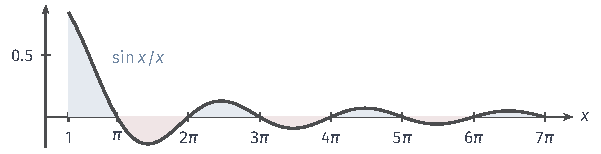
\includegraphics[width=101.699mm]{figures/02-abstract-mathematics/01-metric-and-measure/tikz/c3-sinc-improper/figure.pdf}
 \caption{$f(x)=\sin x/x$在$[1,7\pi]$上的图像，正瓣为蓝、负瓣为红。第$k$瓣$[k\pi,(k+1)\pi]$上$|f|$的面积不小于$2/((k+1)\pi)$，各瓣面积之和按调和级数发散，所以$f$在$[1,+\infty)$上不Lebesgue可积；按$x$增大的次序累加时正负瓣相互抵消，反常积分收敛。}
 \label{fig:integral-sinc-improper}
\end{figure}

\paragraph{Cauchy主值}
在内部奇点两侧，还有一种更依赖次序的规定。$f(x)=1/x$在$[-1,1]\setminus\{0\}$上，两侧同步截断得
\[
 \lim_{\varepsilon\downarrow0}\Bigl(\int_{-1}^{-\varepsilon}\frac{\mathrm dx}x+\int_\varepsilon^1\frac{\mathrm dx}x\Bigr)=\lim_{\varepsilon\downarrow0}(\log\varepsilon-\log\varepsilon)=0,
\]
这称为\term{Cauchy主值}（Cauchy principal value）。若右侧改为从$2\varepsilon$截断，同样的计算得到$\log\varepsilon-\log(2\varepsilon)=-\log2$，可见结果取决于两侧逼近的速度之比。通常的反常积分要求两侧分别取极限，而$\int_\varepsilon^1\mathrm dx/x=-\log\varepsilon\to+\infty$，所以它发散；Lebesgue积分中$\int f^+=\int f^-=+\infty$，积分不存在。主值是在特定问题中额外指定的抵消规则，不能当作反常积分或Lebesgue积分的值。
